\section{Установка Debian GNU/Linux в VirtualBox} \label{pril:b}

\begin{figure}[ht]
    \centering
    \fbox{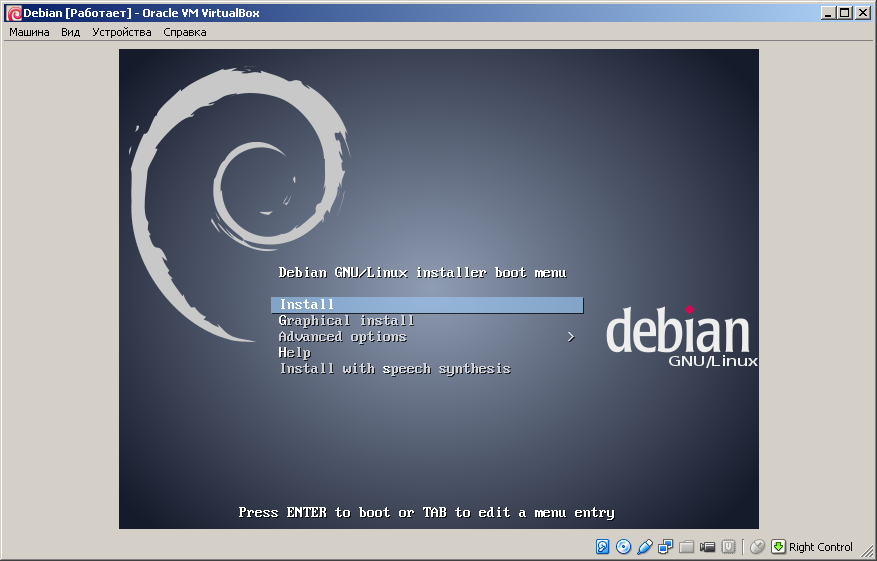
\includegraphics[width=0.75\linewidth]{Screenshot-13}}
    \fbox{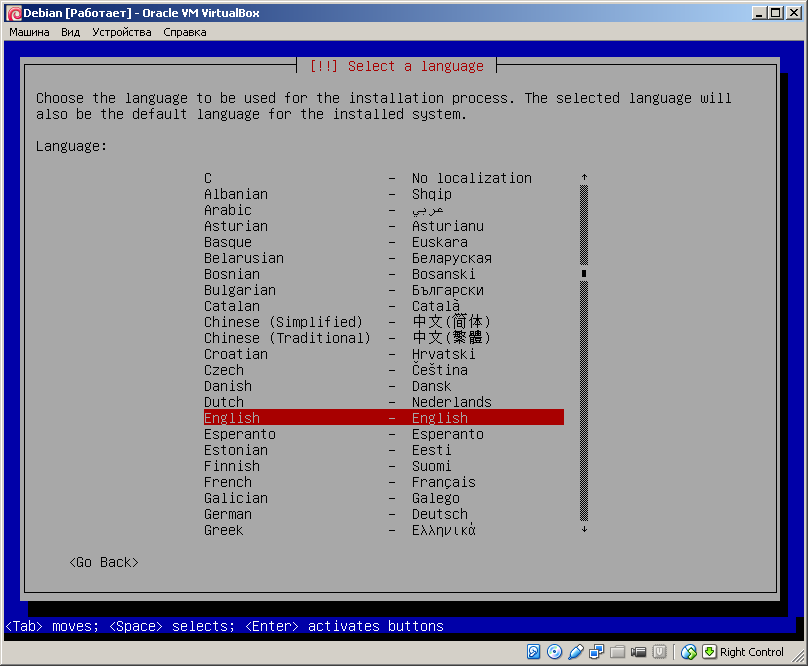
\includegraphics[width=0.75\linewidth]{Screenshot-14}}
\end{figure}

\begin{figure}[ht]
    \centering
    \fbox{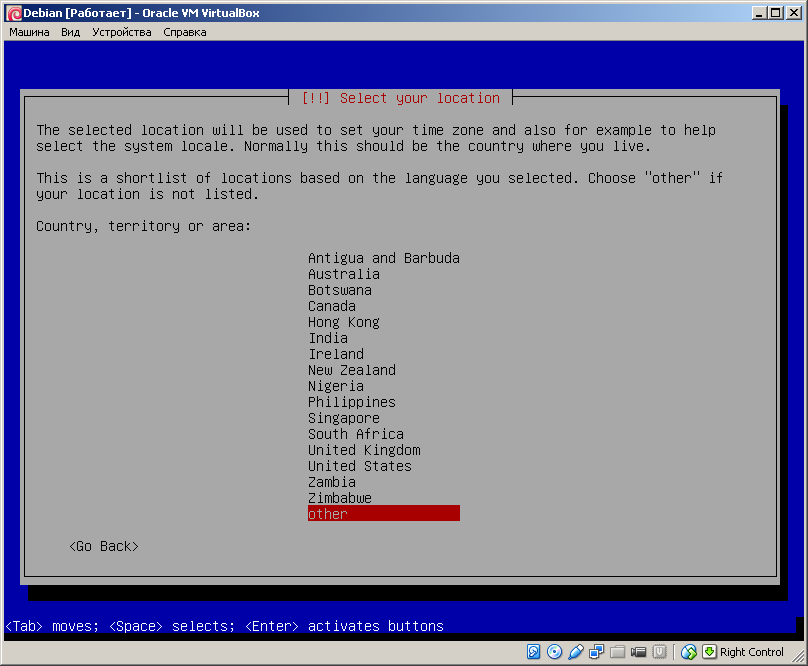
\includegraphics[width=0.9\linewidth]{Screenshot-15}}
    \fbox{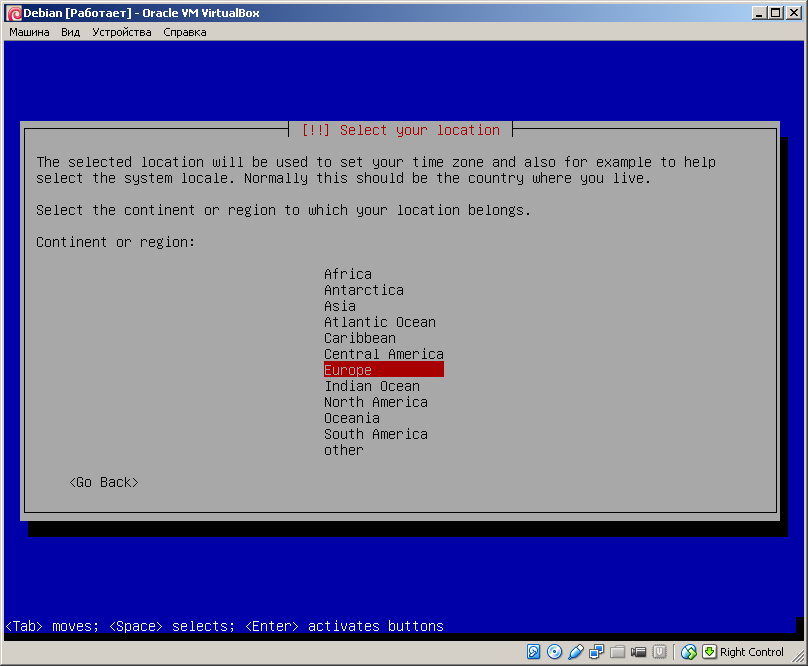
\includegraphics[width=0.9\linewidth]{Screenshot-16}}
\end{figure}

\begin{figure}[ht]
    \centering
    \fbox{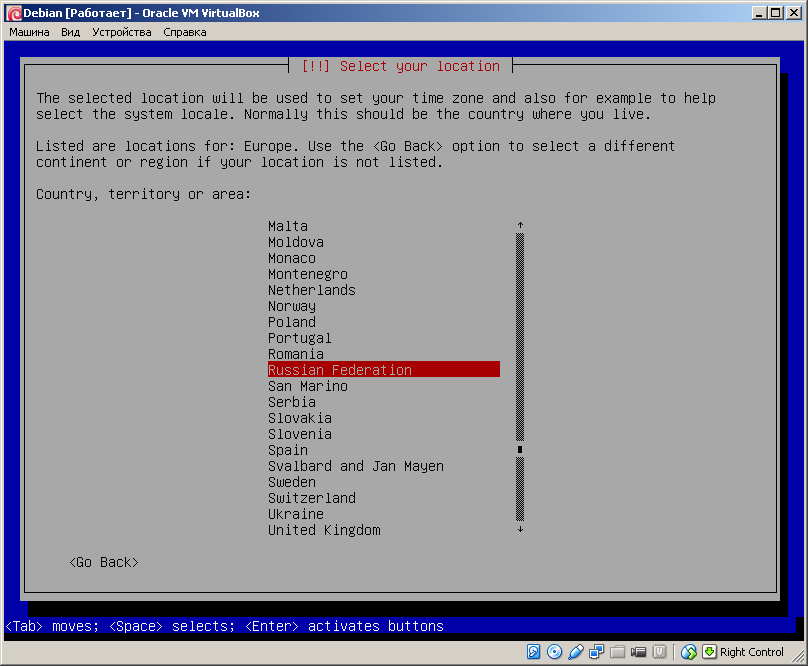
\includegraphics[width=0.9\linewidth]{Screenshot-17}}
    \fbox{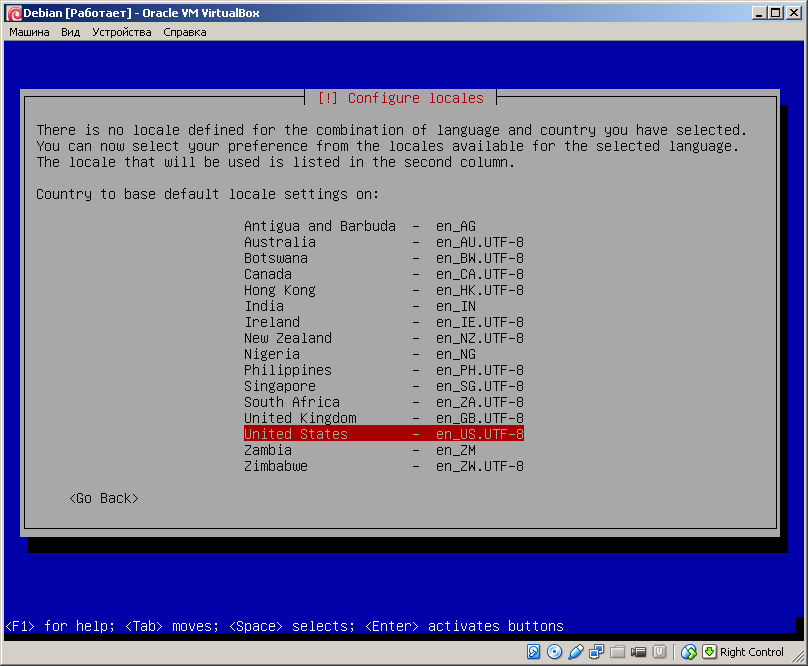
\includegraphics[width=0.9\linewidth]{Screenshot-18}}
\end{figure}

\begin{figure}[ht]
    \centering
    \fbox{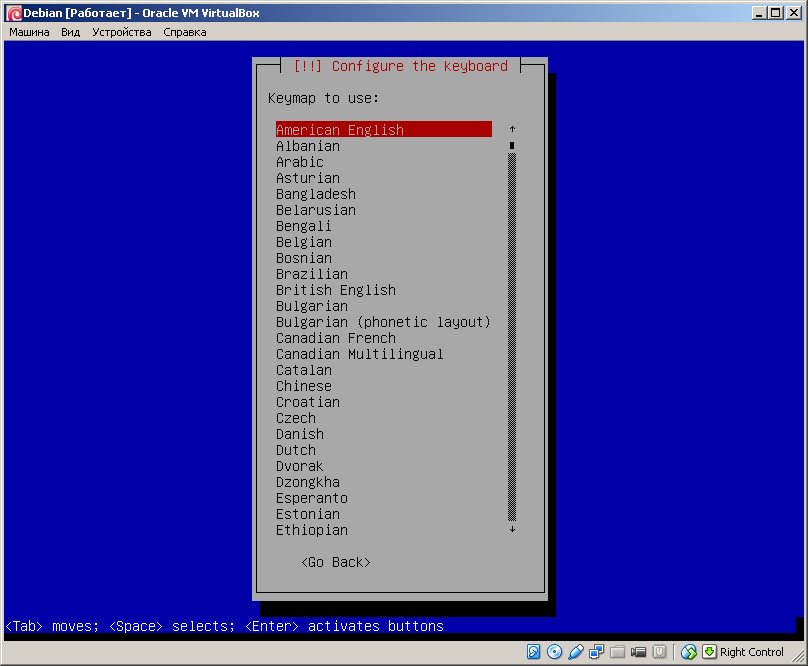
\includegraphics[width=0.9\linewidth]{Screenshot-19}}
    \fbox{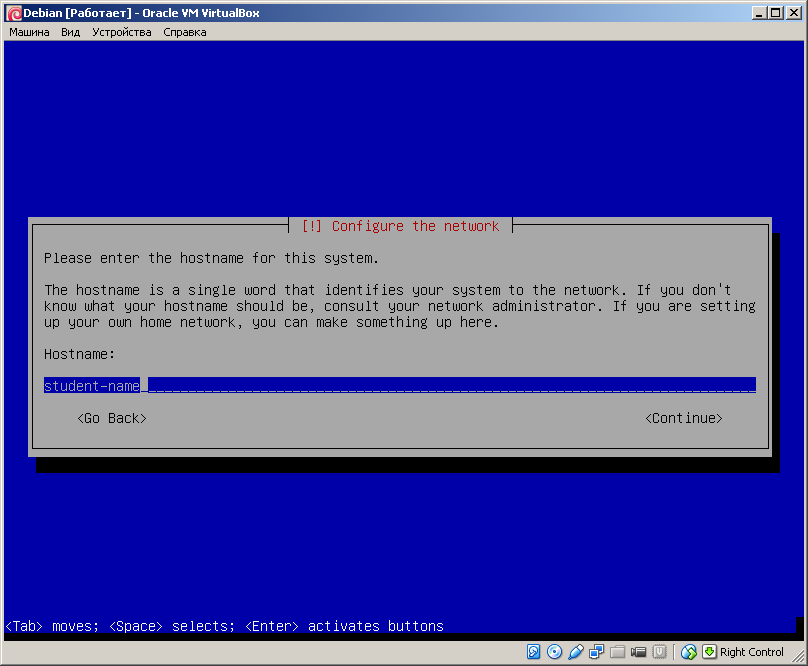
\includegraphics[width=0.9\linewidth]{Screenshot-20}}
\end{figure}

\begin{figure}[ht]
    \centering
    \fbox{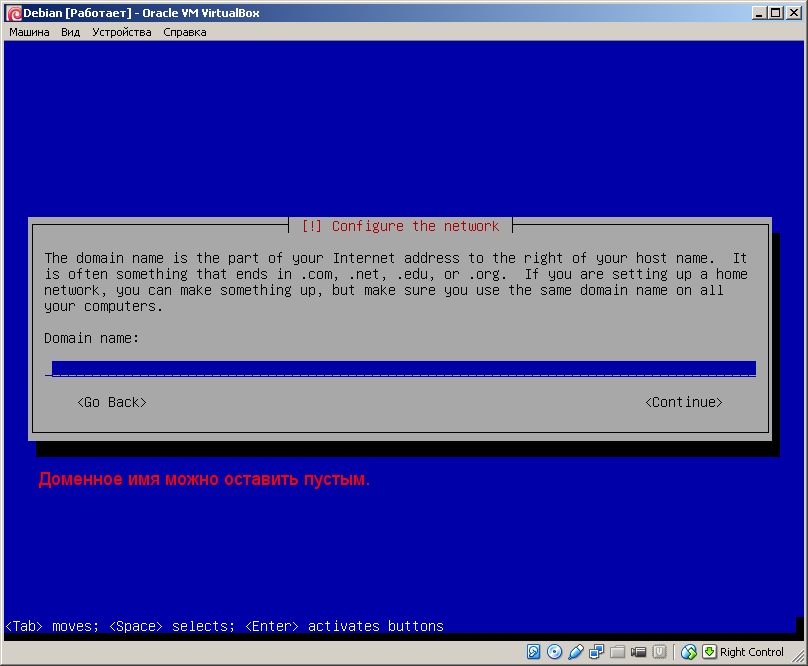
\includegraphics[width=0.9\linewidth]{Screenshot-21}}
    \fbox{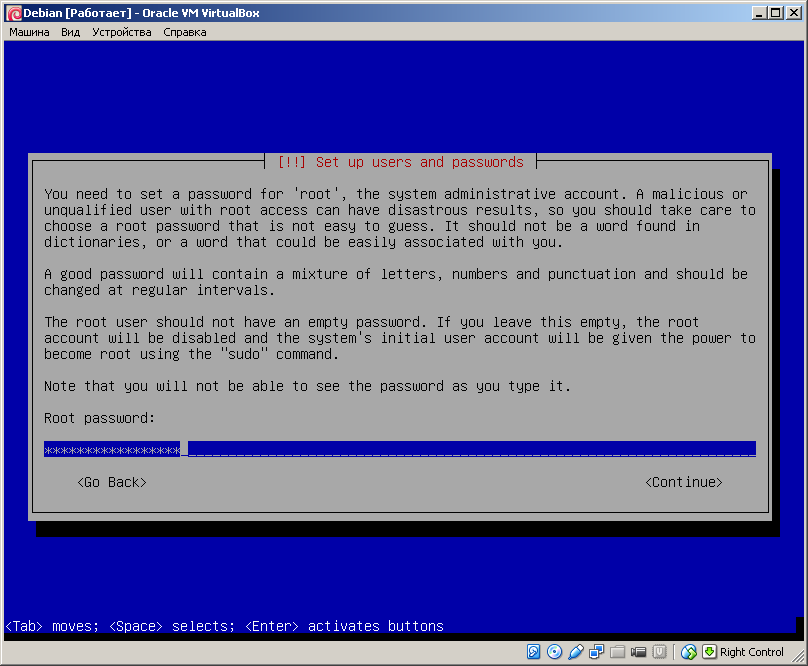
\includegraphics[width=0.9\linewidth]{Screenshot-22}}
\end{figure}

\begin{figure}[ht]
    \centering
    \fbox{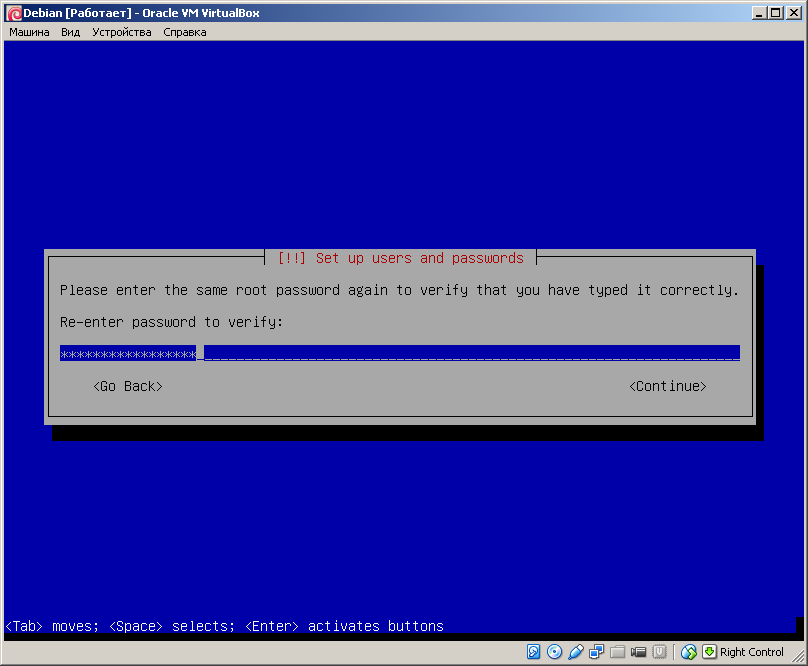
\includegraphics[width=0.9\linewidth]{Screenshot-23}}
    \fbox{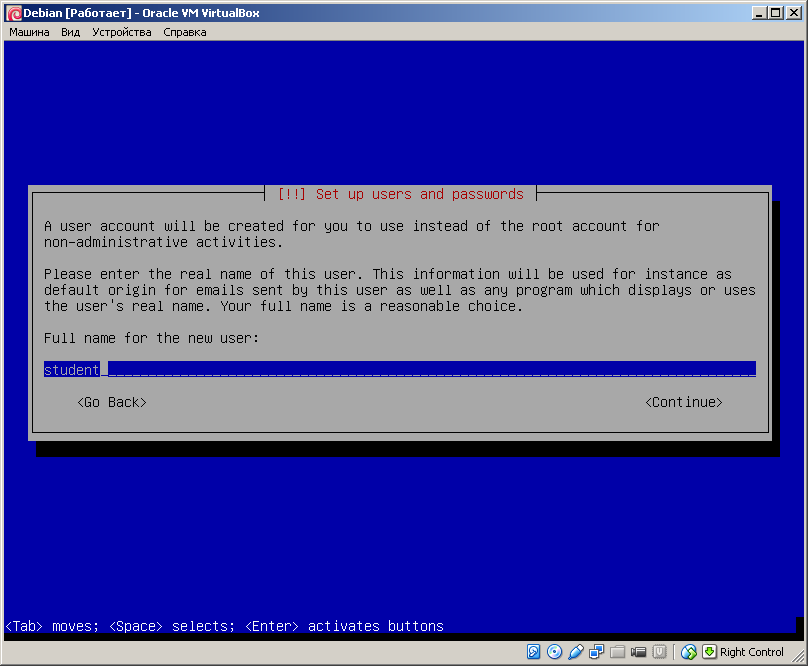
\includegraphics[width=0.9\linewidth]{Screenshot-24}}
\end{figure}

\begin{figure}[ht]
    \centering
    \fbox{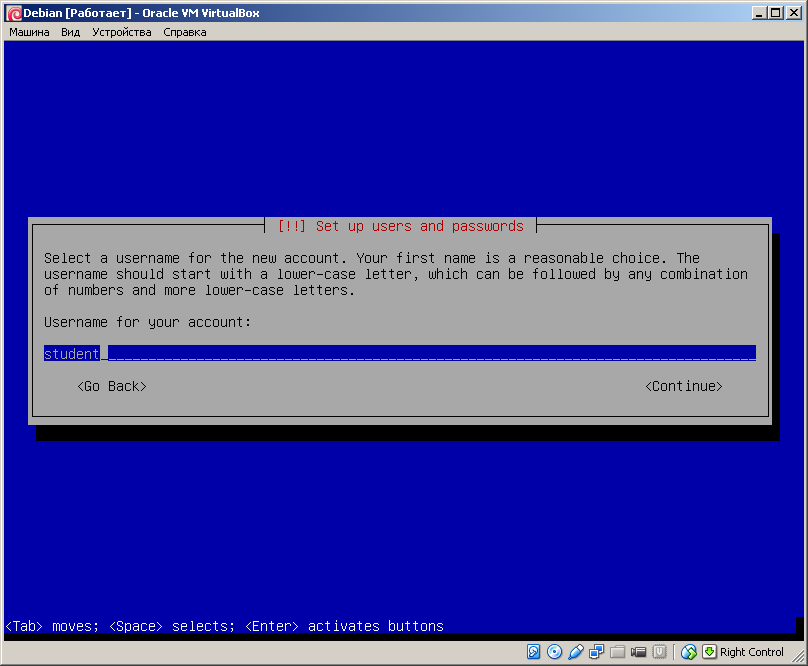
\includegraphics[width=0.9\linewidth]{Screenshot-25}}
    \fbox{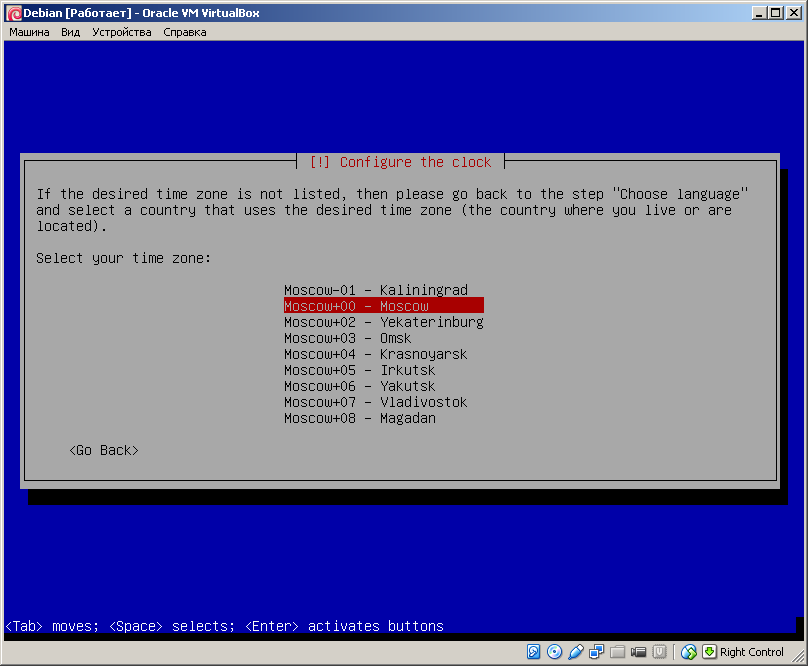
\includegraphics[width=0.9\linewidth]{Screenshot-26}}
\end{figure}


\begin{figure}[ht]
    \centering
    \fbox{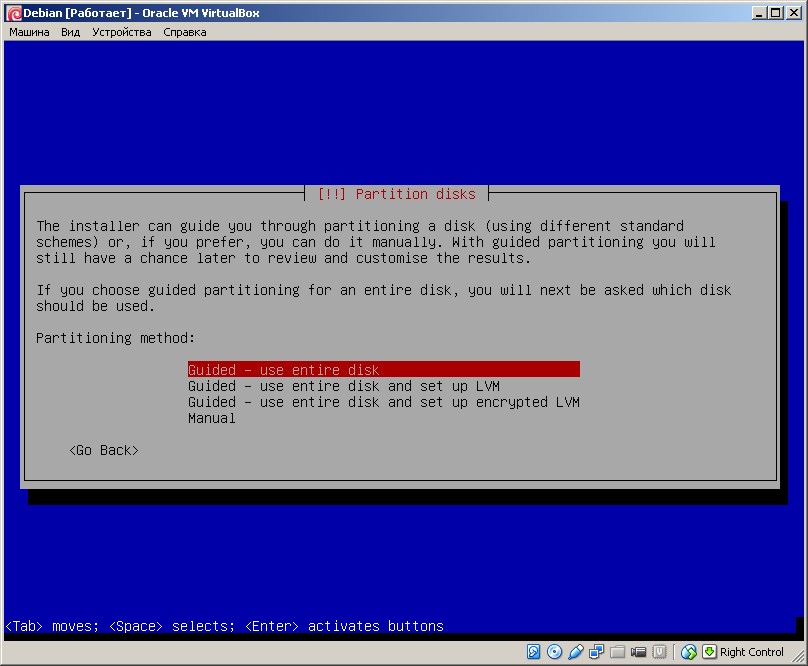
\includegraphics[width=0.9\linewidth]{Screenshot-27}}
    \fbox{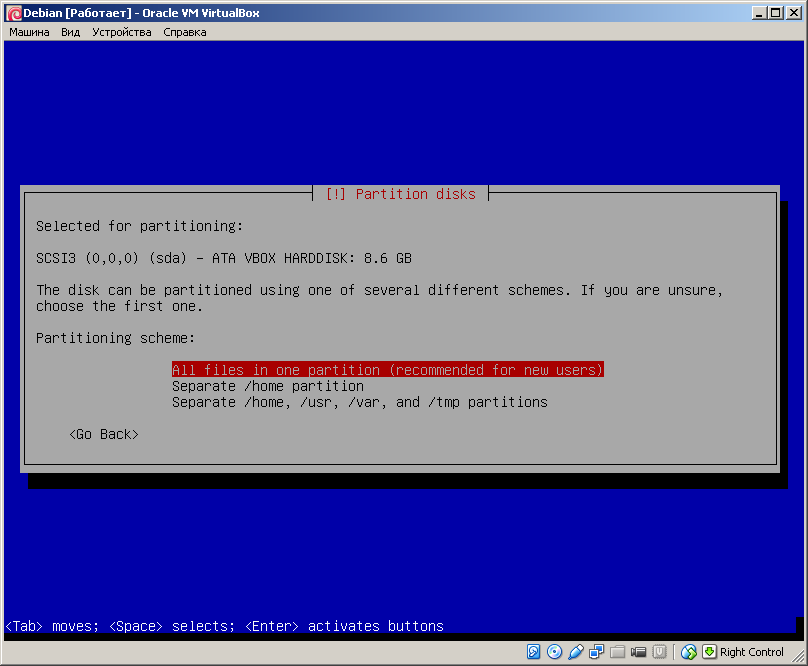
\includegraphics[width=0.9\linewidth]{Screenshot-28}}
\end{figure}

\begin{figure}[ht]
    \centering
    \fbox{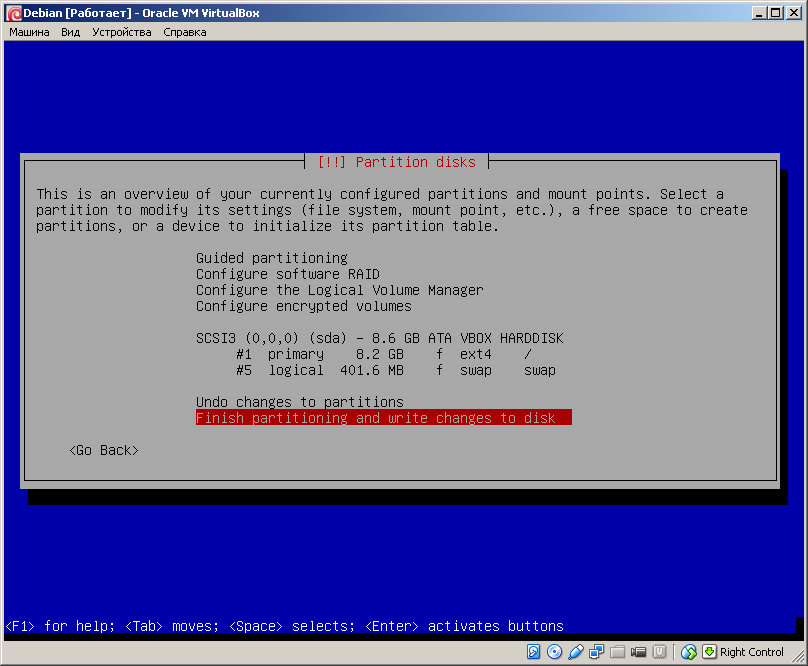
\includegraphics[width=0.9\linewidth]{Screenshot-29}}
    \fbox{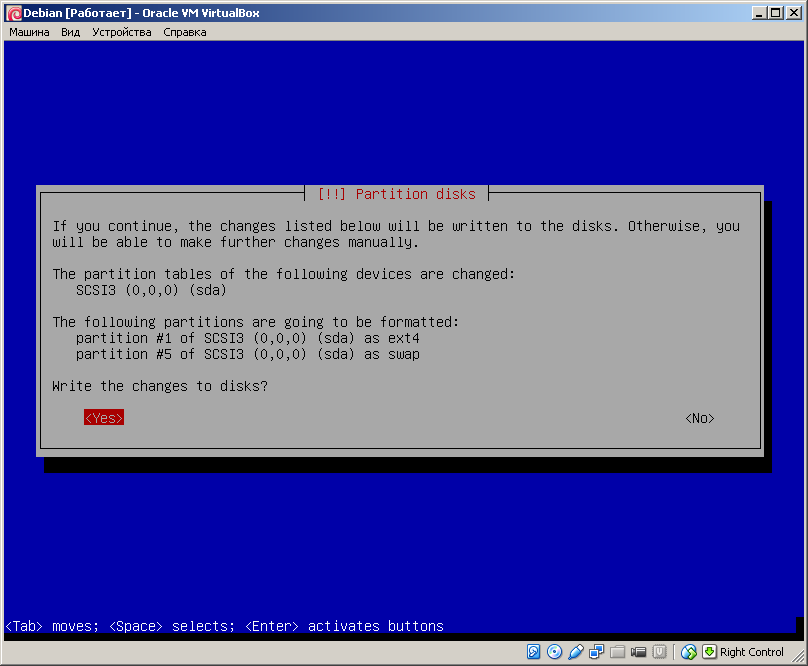
\includegraphics[width=0.9\linewidth]{Screenshot-30}}
\end{figure}

\begin{figure}[ht]
    \centering
    \fbox{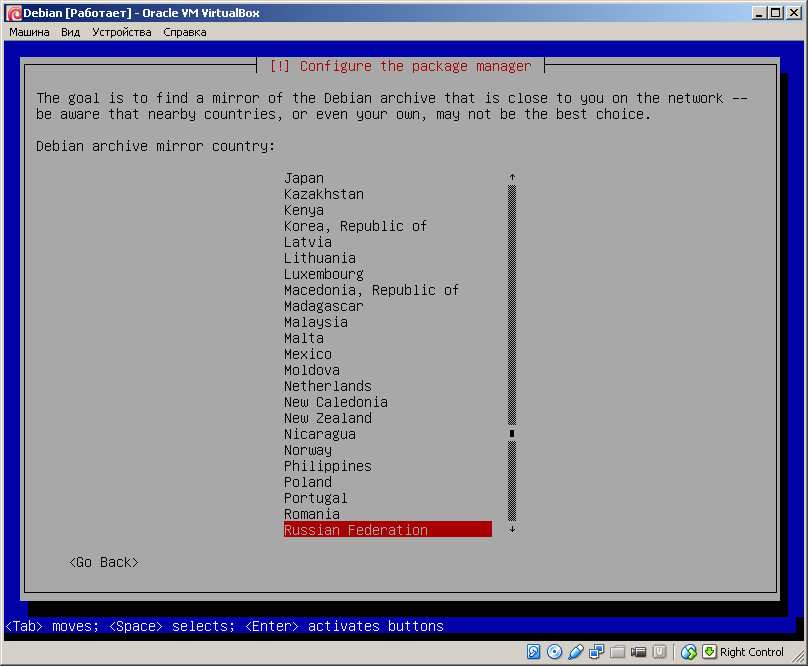
\includegraphics[width=0.9\linewidth]{Screenshot-31}}
    \fbox{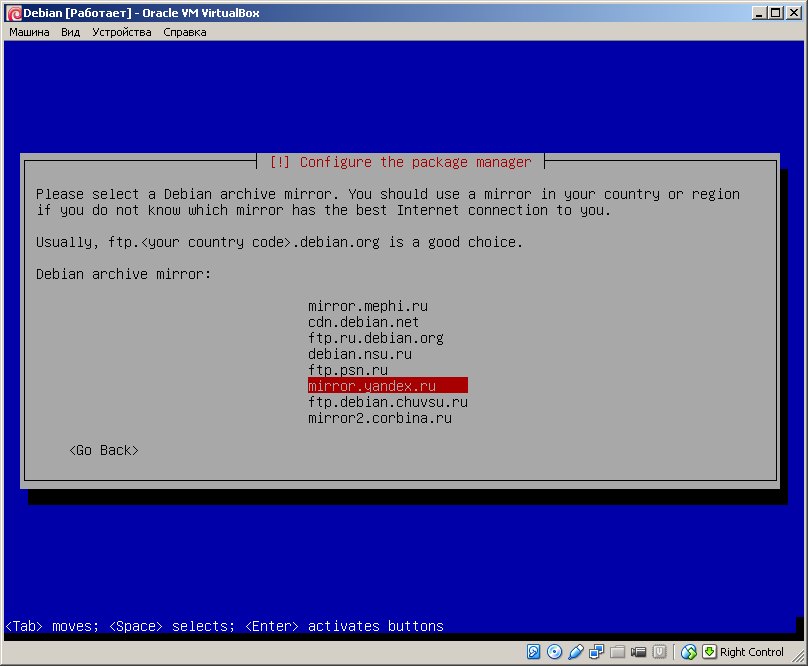
\includegraphics[width=0.9\linewidth]{Screenshot-32}}
\end{figure}

\begin{figure}[ht]
    \centering
    \fbox{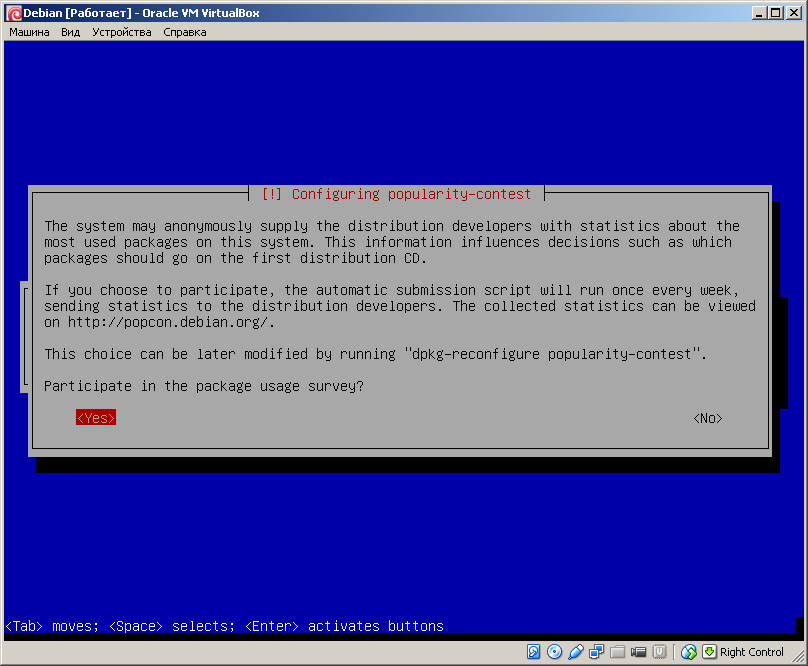
\includegraphics[width=0.9\linewidth]{Screenshot-33}}
    \fbox{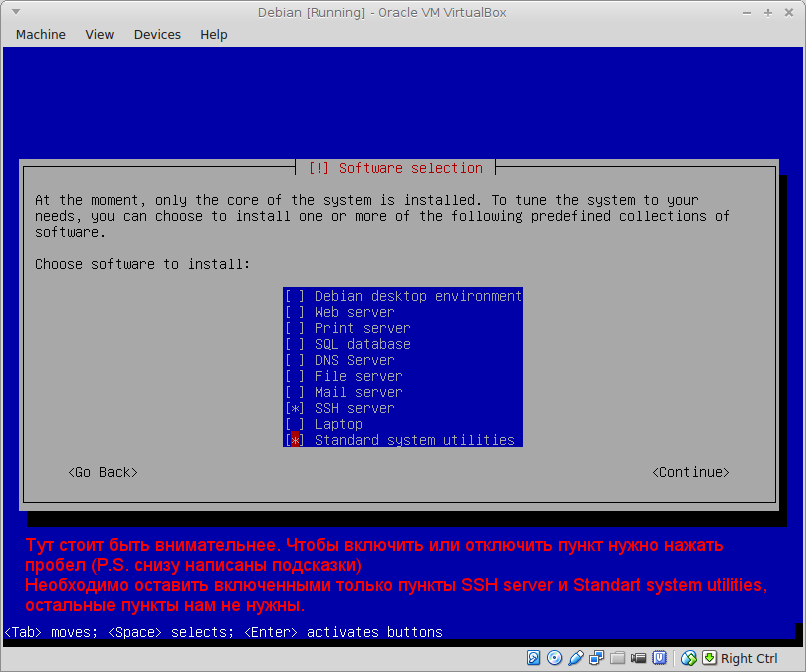
\includegraphics[width=0.9\linewidth]{Screenshot-34}}
\end{figure}

\begin{figure}[ht]
    \centering
    \fbox{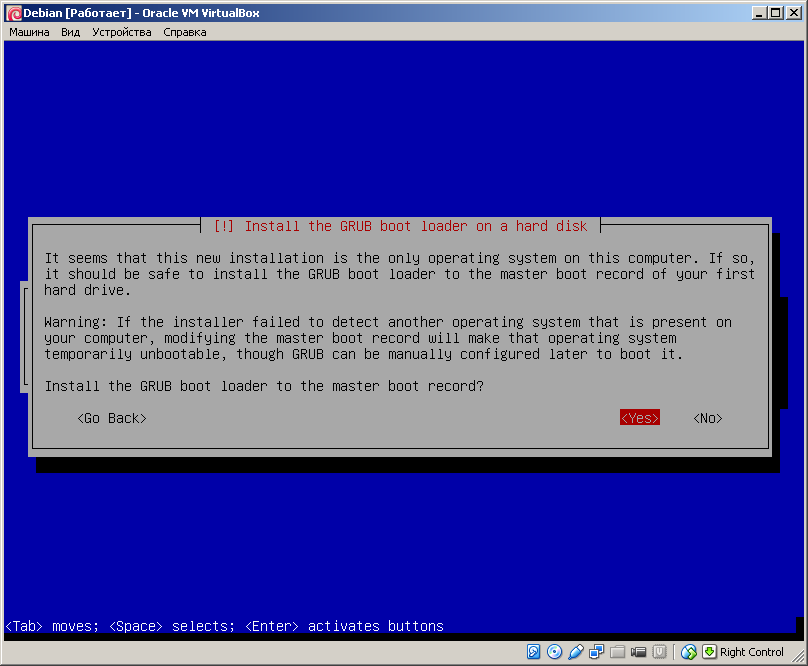
\includegraphics[width=0.9\linewidth]{Screenshot-35}}
    \fbox{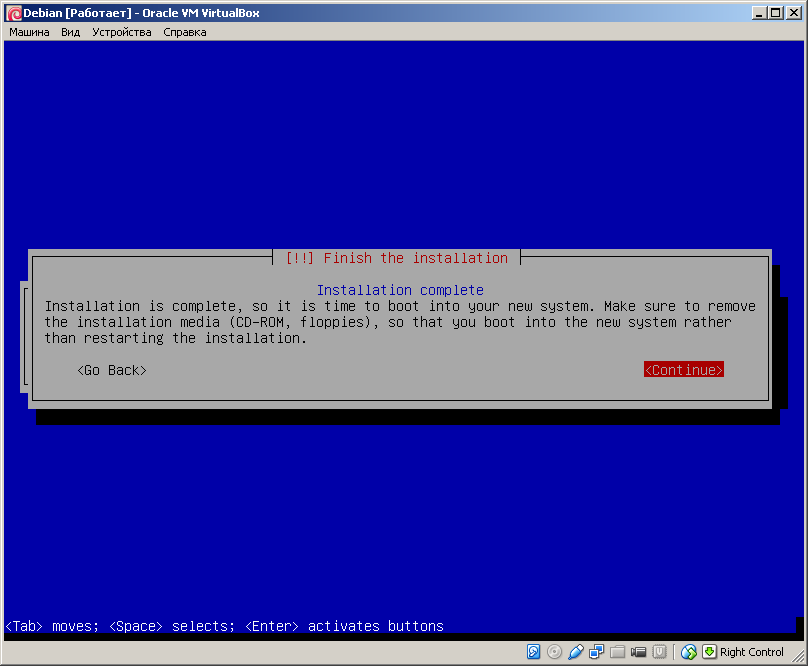
\includegraphics[width=0.9\linewidth]{Screenshot-36}}
\end{figure}

\clearpage

Если после установки, операционная система не получает автоматические настройки сети через DHCP, то необходимо сконфигурировать сеть вручную.

В первую очередь необходимо убедиться, что у сетевого адаптера в настройках виртуальной машины выставлен режим "Сетевой мост".
Затем с помощью команды \texttt{ipconfig} в Windows или \texttt{ifconfig} в Linux/MacOS необходимо узнать параметры своей сети на хост-компьютере.
\begin{figure}[ht]
    \centering
    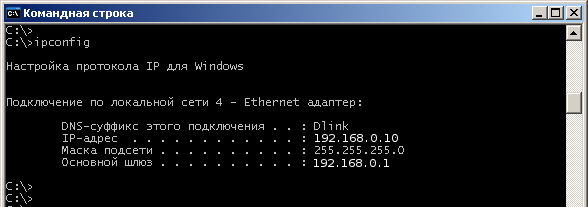
\includegraphics[width=0.9\linewidth]{ipconfig}
    \caption{Настройки сети на хост-компьютере с Windows}\label{pic:ipconfig}
\end{figure}

Тут видно, что хост-компьютер находится в сети \texttt{192.168.0.0}, имеет IP-адрес \texttt{192.168.0.10}, шлюзом является маршрутизатор с IP-адресом \texttt{192.168.0.1}.

Настроим сетевой интерфейс для виртуальной машины вручную, пусть IP-адрес виртуальной машины будет \texttt{192.168.0.102}.
Для этого необходимо отредактировать конфигурационный файл сети и привести его к такому виду:
\begin{lstlisting}
# nano /etc/network/interfaces
source /etc/network/interfaces.d/*
auto lo
iface lo inet loopback

auto eth0
iface eth0 inet static
address 192.168.0.102
netmask 255.255.255.0
network 192.168.0.0
broadcast 192.168.0.255
gateway 192.168.0.1
dns-nameservers 192.168.0.1 8.8.8.8
\end{lstlisting}

В данном конфигурационном файле указаны настройки для основного интерфейса сети (eth0).
После сохранения изменений в конфигурационном файле, необходимо перезапустить демон сети:
\begin{lstlisting}
# /etc/init.d/networking restart
\end{lstlisting}

Проверим на виртуальной машине новые настройки сети:
\begin{lstlisting}
# ip -4 addr show eth0
2: eth0: <BROADCAST,MULTICAST,UP,LOWER_UP> mtu 1500 qdisc pfifo_fast state UP group default qlen 1000
    inet 192.168.0.102/24 brd 192.168.0.255 scope global eth0
       valid_lft forever preferred_lft forever
\end{lstlisting}

Для проверки работы сети пробуем пропинговать адрес \texttt{192.168.0.102} или соединиться к виртуальной машине по ssh.

\clearpage
